% Preamble
\documentclass[11pt]{article}

% Packages
\usepackage[spanish]{babel}
\usepackage{graphicx}

\graphicspath{{images}}

\title{Bases de Datos II \\ \large Proyecto Final}
\author{D'Autilio Joel \and Pablo Rossi}

% Document
\begin{document}

\maketitle
% \tableofcontents

\section{Estructura}

El proyecto consta de tres paquetes principales:

\begin{itemize}
	\item \textit{structure} contiene clases que representan entidades de una base de datos, como \textit{Table}, \textit{Column} o \textit{Procedure}.
	      Un diagrama de este paquete se puede ver en la figura~\ref{fig:uml}
	\item \textit{loader} contiene la clase abstracta \textit{Loader} la cual implementa el método \textit{loadSchema} para cargar el esquema dado en un objeto de tipo \textit{Schema}
	\item \textit{comparator} incluye las clases \textit{DBComparator}, que compara dos esquemas, y \textit{Main}, que contiene el código del programa ejecutable. También incluye el subpaquete \textit{reporter} que genera un reporte a partir del objeto \textit{DBComparator}.
\end{itemize}

\begin{figure}[ht]
	\centering
	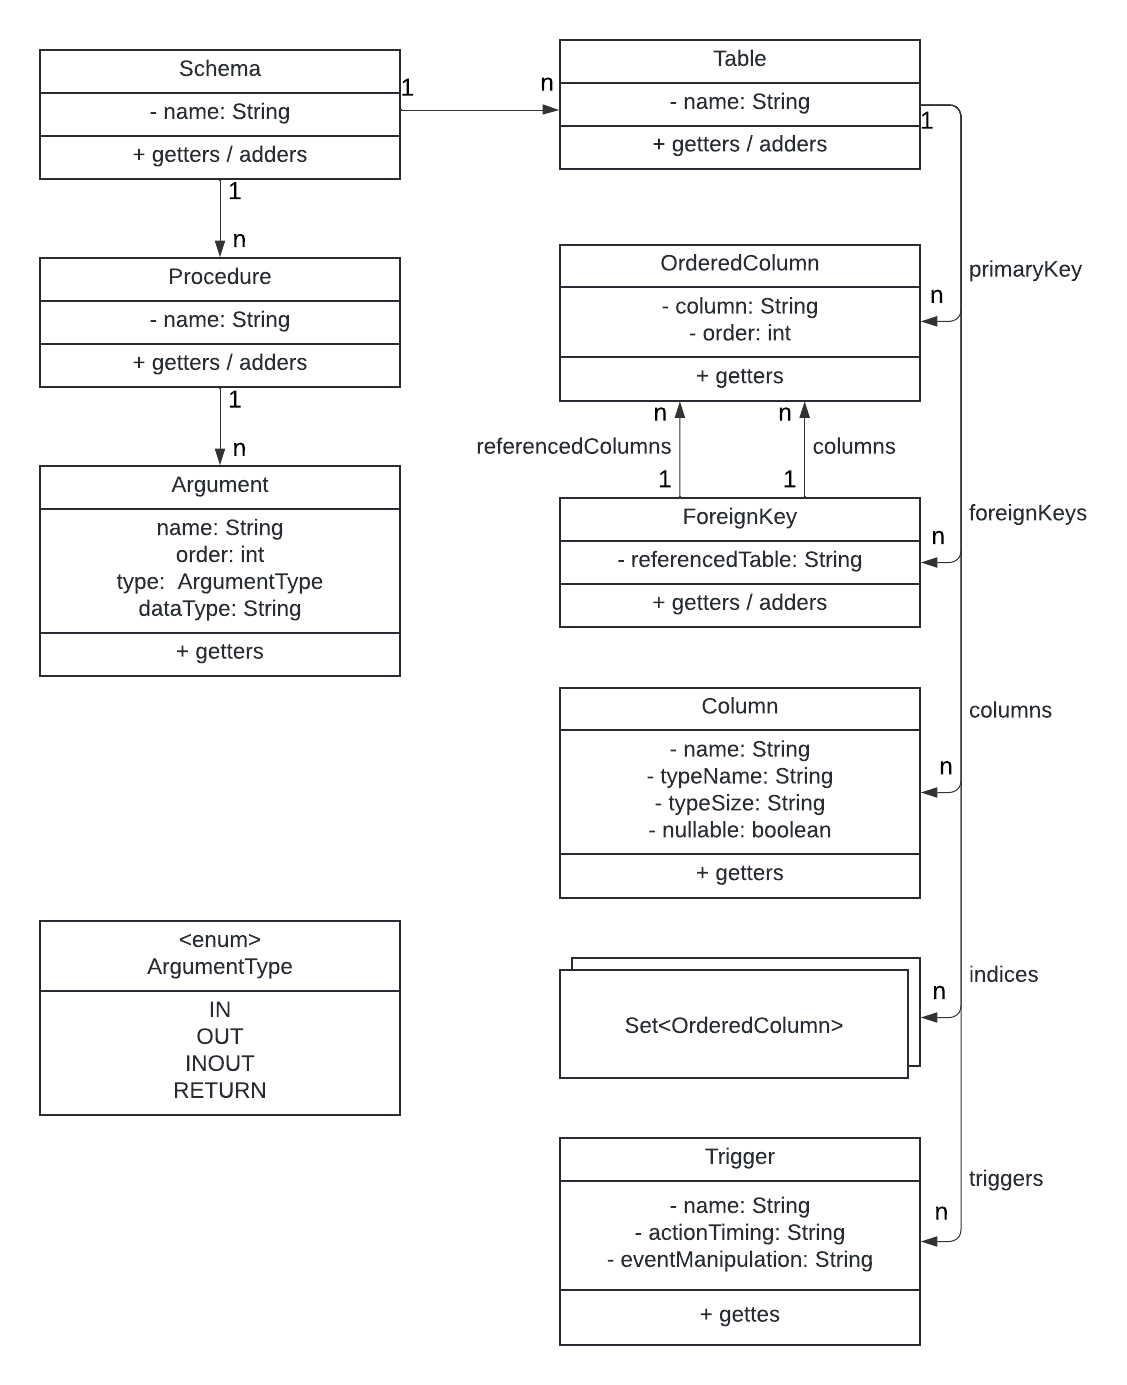
\includegraphics[width=0.9\textwidth]{uml}\label{fig:uml}
	\caption{Diagrama UML de las clases en el paquete \textit{structure}}
\end{figure}


\section{Guía de uso}

El programa se ejecuta en la clase comparator.Main y toma como argumento un archivo de configuración en formato json. Si se pasa un archivo de salida, el reporte se escribe en él. En otro caso, el reporte se escribe en la salida estándar (System.out).

\subsection{Ejemplos de uso}

\begin{itemize}
	\item Escribir el reporte en consola
	      \begin{verbatim*}java comparator.Main config.json\end{verbatim*}
	\item Escribir el reporte en el archivo \textit{output.txt}
	      \begin{verbatim*}java comparator.Main config.json -o output.txt\end{verbatim*}
\end{itemize}


\subsection{Ejemplo de archivo de configuración}

\begin{verbatim}
	> config.json
	{
	    "url": "localhost:3306",    <- URL de la base de datos

	    "catalog1": "db1",          <- Bases de datos a comparar
	    "catalog2": "db2",

	    "username": "usuario",      <- Credenciales de acceso
	    "password": "1234"
	}
\end{verbatim}

\section{Lectura de la salida}

El reporte de salida se divide en dos columnas y cuatro secciones. Cada columna contiene los elementos que tiene una base de datos y la otra no. Las secciones son:

\begin{itemize}
	\item UNIQUE TABLES: Cada columna muestra los nombres de las tablas que son únicas de la respectiva base de datos. Es decir, las tablas que no están presentes en la otra.
	\item COMMON TABLES: Se muestran de a pares las tablas que están presentes en ambas bases de datos. Cada lado incluye los atributos únicos de cada tabla. Los atributos, índices y triggers comunes de ambas tablas no se muestran, sólo las diferencias.
	\item UNIQUE PROCEDURES: Se muestran los procedimientos que son únicos de cada base de datos (por nombre).
	\item COMMON PROCEDURES: Se muestran de a pares los procedimientos que están presentes en ambas bases de datos. Cada columna muestra el procedimiento junto con los argumentos que son únicos. Los argumentos comúnes se simbolizan con el símbolo `\_' (guión bajo).
\end{itemize}

\end{document}
